% Template for ASRU-2015 paper; to be used with:
%          spconf.sty  - ICASSP/ICIP LaTeX style file, and
%          IEEEbib.bst - IEEE bibliography style file.
% --------------------------------------------------------------------------
\documentclass{article}
\usepackage[UTF8, heading = false, scheme = plain]{ctex}
\usepackage{graphicx}
\usepackage{spconf,amsmath,graphicx}
\usepackage{times}
\usepackage{url}
\usepackage{latexsym}
\usepackage{tikz}
\usepackage{bm}
\usepackage{booktabs}
\usepackage{amssymb,amsmath}
\usepackage{relsize}
\usepackage[font={small}]{caption}

\newcommand{\newo}{GESD}
\newcommand{\newt}{AESD}
\newcommand{\todo}[1]{ \textcolor{red}{#1} }
\newcommand{\RN}[1]{%
  \textup{\uppercase\expandafter{\romannumeral#1}}%
}
\usepackage[font={small}]{caption}
\newcounter{magicrownumbers}
\newcommand\rownumber{\stepcounter{magicrownumbers}\arabic{magicrownumbers}}

% Example definitions.
% --------------------
\def\x{{\mathbf x}}
\def\L{{\cal L}}

% Title.
% ------
\title{QA-system \\问答系统}
%
% Single address.
% ---------------

\name{金卓林}
\address{
  哈尔滨工业大学, 150001\\
  {\tt <kimnoic@gmail.com>}
}
%
% For example:
% ------------
%\address{School\\
%	Department\\
%	Address}
%
% Two addresses (uncomment and modify for two-address case).
% ----------------------------------------------------------
%\twoauthors
%  {A. Author-one, B. Author-two\sthanks{Thanks to XYZ agency for funding.}}
%	{School A-B\\
%	Department A-B\\
%	Address A-B}
%  {C. Author-three, D. Author-four\sthanks{The fourth author performed the work
%	while at ...}}
%	{School C-D\\
%	Department C-D\\
%	Address C-D}
%
\begin{document}
%\ninept
%
\maketitle
%


\begin{abstract}
我们应用神经网络框架来解决非实质问题的回答任务。
我们的方法不依赖于其他的语言工具,也可以应用在其他语言领域中。参考了CNN神经网络结构 \cite{adlt}中的第二种。通过测试develop.txt文件,实验结果表明MRR在0.77,并比较了不同训练测试集的次数,最终选择了9000次作为最终结果。

\end{abstract}

%
\begin{keywords}
答案选择,问题回答,卷积神经网络,tensorflow
\end{keywords}
%
\section{介绍}
\label{sec:intro}
自然语言理解为基础的问答系统在过去几年的人工智能领域一直是一个热门话题,许多系统都包括了问答系统例如Siri和Watson等。我们的任务是给出训练集,其中包括问题和问题的答案候选池以及做出最匹配的正确选项,在此基础上给出其他问题和候选答案的相关度。为了找到最佳匹配对,我们需要一个度量来衡量每个QA队的匹配度,以便选择具有最高度量值的QA对。我们先做了一个实验,将问题和答案分词后,用wiki\_cn训练出的词向量进行余弦计算,作为相关度结果。实验表明MRR在0.42,效果不是很好。又阅读了一篇论文\cite{adlt},找到了新的做法。


\section{模型描述}
\label{sec:model}
在这部分将介绍该框架的深度学习框架,以及这个方法的结构。学习给定问题的分布向量及其答案候选,然后是用相似性来度量匹配度。

\subsection{基准系统} 
基准系统是一个字模型,第一步是训练word embedding,被认为是问题中的每个标记及其候选答案的加权和。这就产生了问题和每个候选答案的向量表示,最后一步是计算每个问题和候选对之间的余弦相似度,具有最高余弦相似度的作为答案返回。


\subsection{卷积神经网络框架}
CNN利用三个重要思想可以帮助改进机器学习系统:稀疏的交互,参数共享和等值表示。稀疏的交互与传统的神经网络相反,其中每个输入和输出交互。在CNN中过滤器尺寸通常比输入尺寸小,因此输出与输入的部分窗口交互。参数共享是指在卷积运算中再利用滤波参数,而传统神经网络矩阵中的参数只能使用一次来计算输出。以下是展示CNN实现的一个例子。

\begin{equation}
\label{eq:input_filter}
\small
\left( \begin{array}{cccc}
w_{11} & w_{21} & w_{31} & w_{41} \\
w_{12} & w_{22} & w_{32} & w_{42} \\
w_{13} & w_{23} & w_{33} & w_{43} \end{array}\right)  \bigodot
 \left( \begin{array}{cc}
f_{11} & f_{21}  \\
f_{12} & f_{22}  \\
f_{13} & f_{23} \end{array}
 \right)
\end{equation}
左面的矩阵是输入矩阵,每个单词都是由三维的自向量表示,输入长度为4,右矩阵F表示滤波器。
\begin{equation}
\label{eq:convout}
\small
\begin{aligned}
o_1 &= w_{11}f_{11} + w_{12}f_{12} + w_{13}f_{13} +w_{21}f_{21} + w_{22}f_{22} + w_{23}f_{23} \\ 
o_2 &= w_{21}f_{11} + w_{22}f_{12} + w_{23}f_{13} +w_{31}f_{21} + w_{32}f_{22} + w_{33}f_{23} \\
o_3 &= w_{31}f_{11} + w_{32}f_{12} + w_{33}f_{13} +w_{41}f_{21} + w_{42}f_{22} + w_{43}f_{23} \\
\end{aligned}
\end{equation}
滤波器F将保留最大值,这表示F与W匹配的最好程度。

\subsection{训练和损失函数}
在训练过程中,每个问题都有一个最准确的答案A+,通过将A+和其他错误答案A-配对进行训练。其中深度学习框架中输入为问题、正向答案、负向答案的向量。分别计算问题和两种答案的余弦相似度,并计较二者的差和边界的大小。当满足{\small$cos(V_{Q},V_{A^+}) - cos(V_{Q},V_{A^-}) < m$}~时,表示正向答案排在负向答案后面。满足{\small$cos(V_{Q},V_{A^+}) - cos(V_{Q},V_{A^-}) >= m$}时,则不用更新参数。让正向答案和问题之间的向量cosine值要大于负向答案和问题的向量cosine值,大多少,就是margin这个参数来定义的。cos值越大,两个向量越相近,所以通俗的说这个Loss就是要让正向的答案和问题愈来愈相似,让负向的答案和问题越来越不相似。损失函数为:
\begin{equation}
\small
L = max\left\{0, m - cos(V_{Q},V_{A^+}) +cos(V_{Q},V_{A^-}) \right\}
\end{equation}


\subsection{结构}

Q、A:句子中的每个字都需要转换成对应的字向量\\

%HL:Q中的每个句子会通过HL层的点积进行变换,相当于每个字的自向量从size改变\\
CNN:列大小和字向量大小是一样的,对于每个句子而言,结果是一个列向量,取max-pooling就变成了一个数字,得到了一个句子的语义表示向量。\\

R:是输出结果上加上Relu激活函数\\

最后一层为计算向量的余弦夹角\\

原结构\cite{git}中包含一层隐含层,因为测试效果不佳删去了。\\
\begin{figure}[t]
\begin{center}
\begin{tikzpicture}[scale=0.8]
  \begin{scope}
    \draw (1.6,0.0)rectangle (2.0,1.2) node[pos=.5] {\scriptsize A};  
    \draw (1.6,1.8)rectangle (2.0,3.0) node[pos=.5] {\scriptsize Q};   
    %\draw (0.8,0.0)rectangle (2.0,3.0) node[pos=.5] {\scriptsize HL$_{QA}$};   
    \draw (2.5,0.0)rectangle (3.7,3.0) node[pos=.5] {\scriptsize CNN$_{QA}$};
    \draw (4.0,0.0)rectangle (4.4,1.2) node[pos=.5] {\scriptsize \begin{tabular}{c} P \\ $+$ \\ R \end{tabular}};
    \draw (4.0,1.8)rectangle (4.4,3.0) node[pos=.5] {\scriptsize \begin{tabular}{c} P \\ $+$ \\ R \end{tabular}};
    
    %\draw [->, thick] (0.4,0.6) -- (0.8,0.6);
    \draw [->, thick] (2.0,0.6) -- (2.5,0.6);
    %\draw [->, thick] (0.4,2.4) -- (0.8,2.4);
    \draw [->, thick] (2.0,2.4) -- (2.5,2.4);
    \draw [->, thick] (3.7,0.6) -- (4.0,0.6);
    \draw [->, thick] (3.7,2.4) -- (4.0,2.4);
    \draw [->, thick] (4.4,0.6) -- (5.2,1.4);
    \draw [->, thick] (4.4,2.5) -- (5.2,1.8);
    \fill (5.5,1.6) circle[radius=1pt] ;
    \draw (5.5,1.6) circle[radius=10pt, thick];
    \node at (5.5,2.4) {\scriptsize 余弦};
    \node at (5.7,2.1) {\scriptsize 相似度};
  \end{scope}
\end{tikzpicture}
\end{center}
\label{fig:arc2}
\end{figure}




\section{实验情况}
我们将上文提到的神经网络结构,使用python下的tensorflow库实现并用老师提供的数据集和开发集进行开发、用测试集进行测试。Tensorflow工具集提供了深度学习所需要的大部分常用数据结构和函数的支持,此次未使用其他工具集。\\

我们部署的神经网络部分包括word embedding层,卷积-MaxPooling层和输出层\\

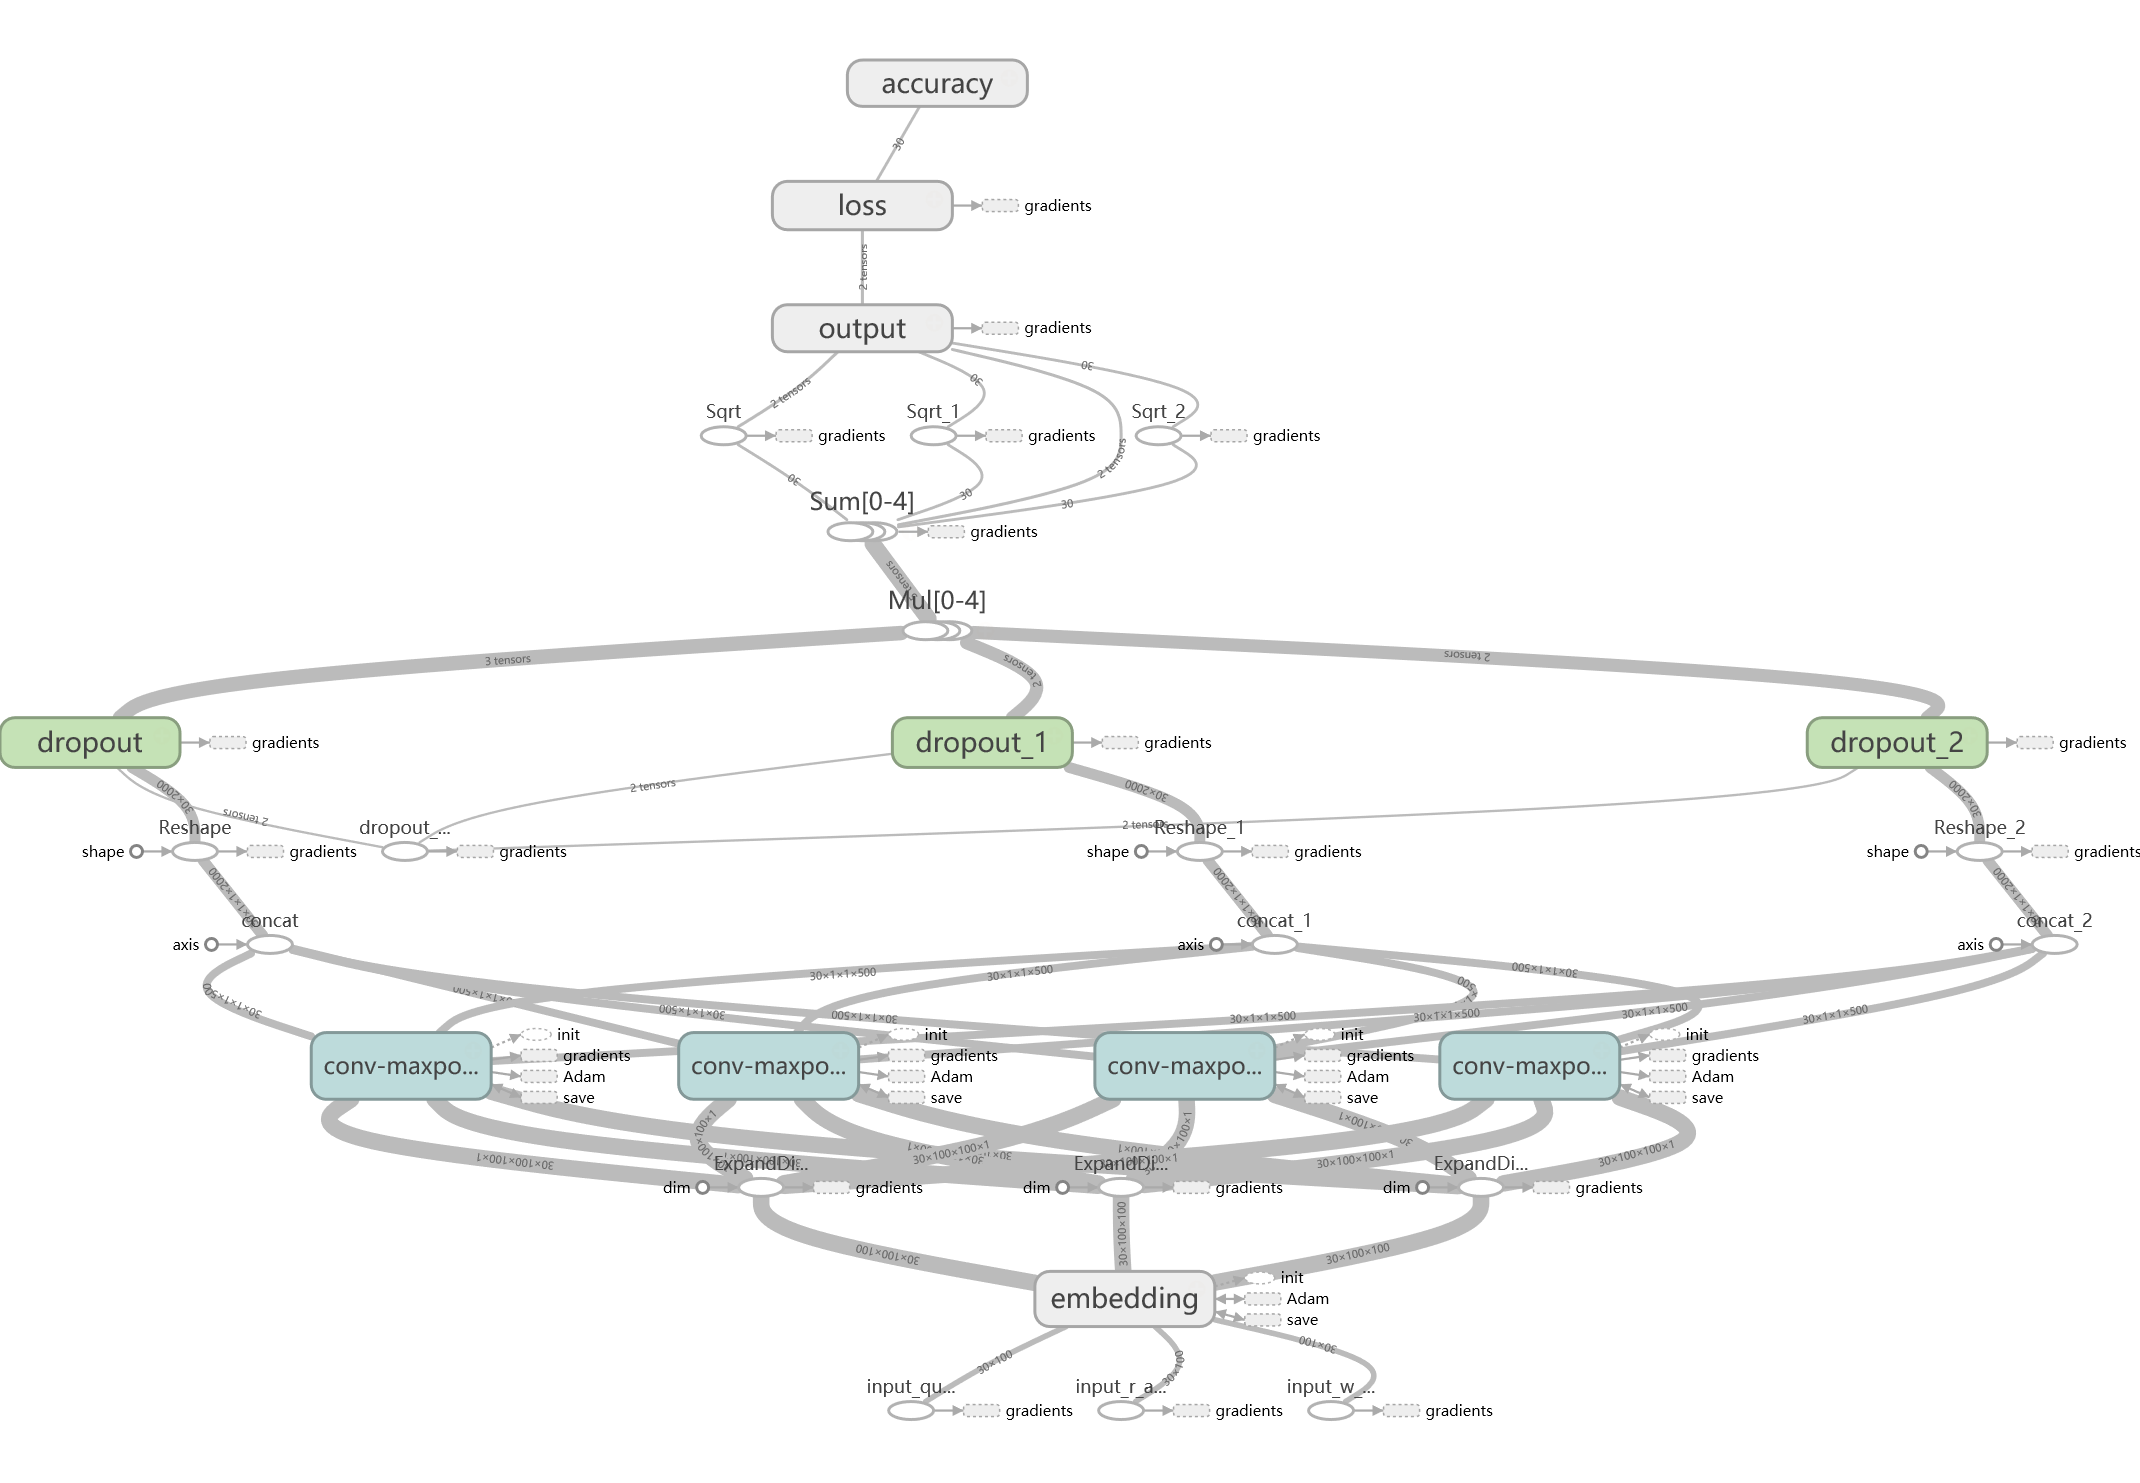
\includegraphics[height=160]{1.png}\\

上图为tensorflow下构建的神经网络的数据流图\\

其中word embedding时采用100维空间,并且每个字word embedding结果也是可优化参数。CNN采用4个filter,filter大小分别为1、3、4、5。MaxPooling后输入项转换为2000维向量,输出层将三个输入项(问题,正向回答,负向回答)经过前两层得到的向量按照前述的方法计算余弦相似度,并取m=0.05按照前述公式计算损失函数L。\\

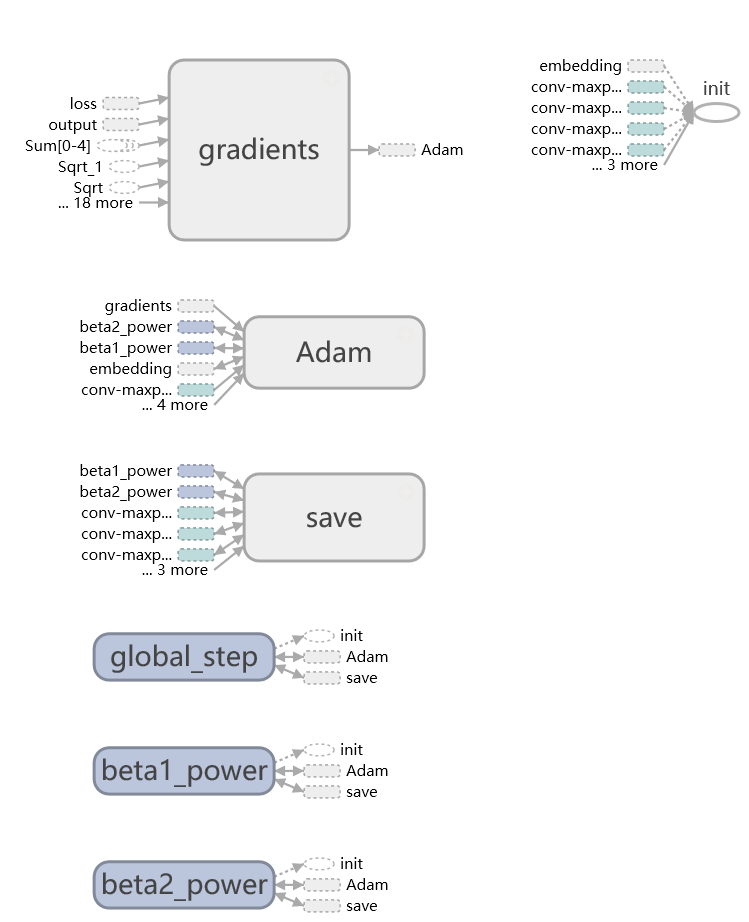
\includegraphics[height=300]{2.png}\\

在训练时,利用tensorflow的feed机制,从训练集中随机选择30个问题,然后每个问题随机选择一个正向回答和负向回答(如果没有负向回答则随机选择一个无关回答)作为一个批次(batch),参数的优化采用内建的Adam优化器\cite{adam},learning rate为0.1。在回答时,传入问题和待选答案,根据输出层中问题和答案的余弦相似度作为答案的权重。
\section{总结}
最后时间比较仓促没有对迭代次数进行分析,可能会造成结果不同的影响。估计了一个大致收敛的位置,并对小规模数据测试,最终决定了迭代次数。\\

通过这次比赛,还是学到了不少新的知识,包括对QAsystem、CNN的理解和tensorflow的简单使用。








% To start a new column (but not a new page) and help balance the last-page
% column length use \vfill\pagebreak.
% -------------------------------------------------------------------------
%\vfill
%\pagebreak


% References should be produced using the bibtex program from suitable
% BiBTeX files (here: strings, refs, manuals). The IEEEbib.bst bibliography
% style file from IEEE produces unsorted bibliography list.
% -------------------------------------------------------------------------
\newpage
\bibliographystyle{IEEEbib}
\bibliography{Template}

\end{document}
